

\subsection{Output Analysis of $S(R)$}
      
      \begin{figure}
        \centering
        
        \begin{subfigure}[b]{0.45\textwidth}
          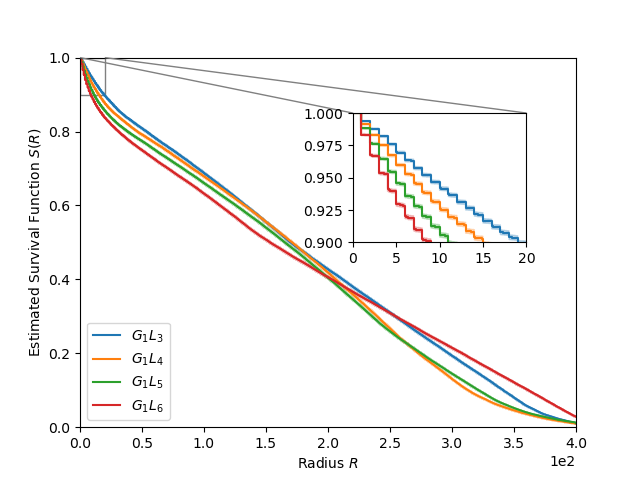
\includegraphics[width=\textwidth]{G_1_initial_radius_sf.png}
          \caption{}
          \label{fig:sf_g1_branch_radius}
        \end{subfigure}
        \hfill
        \begin{subfigure}[b]{0.45\textwidth}
          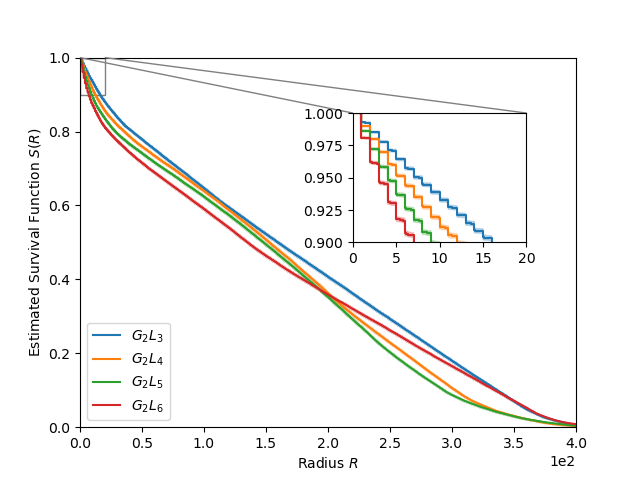
\includegraphics[width=\textwidth]{G_2_initial_radius_sf.png}
          \caption{}
          \label{fig:sf_g2_branch_radius}
        \end{subfigure}

        \caption{}
        \label{fig:sf_branch_radius}

      \end{figure}

      
      \begin{table}
        \centering
        \begin{tabular}{llrrrr}
          \toprule
                       &             &         &  p &    &     \\
          \cmidrule{3-6}
                       &             & Logrank & TW & GB & FH  \\
          \midrule
          $G_1$ $L_3$  & $G_1$ $L_4$  &  0.0 &  0.0 &  0.0 &  0.0     \\
                       & $G_1$ $L_5$  & 0.0 & 0.0 & 0.0 & 0.0    \\
                       & $G_1$ $L_6$  & 0.0 & 0.0 & 0.0 & 0.0      \\
          $G_1$ $L_4$  & $G_1$ $L_5$  & 0.1773 & 0.0 & 0.0 & 0.0      \\
                       & $G_1$ $L_6$  & 0.0 & 0.0 & 0.0 & 0.0       \\
          $G_1$ $L_5$   & $G_1$ $L_6$ & 0.0 &  0.0 & 0.0 & 0.0      \\
          \bottomrule
        \end{tabular}
        \label{tab:g1_ingroup_tests_radius}
        \caption{}
      \end{table}


      \begin{table}
        \centering
        \begin{tabular}{llrrrr}
          \toprule
                       &             &         &  p &    &     \\
          \cmidrule{3-6}
                       &             & Logrank & TW & GB & FH  \\
          \midrule
          $G_2$ $L_3$  & $G_2$ $L_4$  &  0.0 &  0.0 &  0.0 &  0.0     \\
                       & $G_2$ $L_5$  & 0.0 & 0.0 & 0.0 & 0.0    \\
                       & $G_2$ $L_6$  & 0.0 & 0.0 & 0.0 & 0.0      \\
          $G_2$ $L_4$  & $G_2$ $L_5$  & 0.0 & 0.0 & 0.0 & 0.0      \\
                       & $G_2$ $L_6$  & 0.0 & 0.0 & 0.0 & 0.0       \\
          $G_2$ $L_5$   & $G_2$ $L_6$ & 0.0 & 0.0 & 0.0253 & 0.0253      \\
          \bottomrule
        \end{tabular}
        \label{tab:g2_ingroup_tests_radius}
        \caption{}
      \end{table}


      

















